\chapter{Implementierung} \label{chap:implementierung}

\section{Backend-Server}

\subsection{Verwendete Technologien} \label{sec:impl-server-technology}

Die grundlegend verwendete Technologie für den Backend-Server ist die Programmiersprache \enquote{Go}.
Go wurde ausgewählt, da es eine einfach zu verstehende Programmiersprache ist, die optimiert für Server-Anwendungen ist (vgl. \cite{Weigend2019}).
Zudem sind alle am Projekt beteiligten Personen schon mit der Sprache vertraut.

Go stellt eine gute Standardbibliothek zur Verfügung, die an vielen Stellen verwendet wird.
Trotzdem werden zusätzlich einige externe Bibliotheken verwendet.
Diese dienen hauptsächlich dazu, die externen Schnittstellen (\gls{HTTP} und \gls{CoAP}) mit den dazugehörigen Datenformaten zur Verfügung zu stellen.
Auch werden Bibliotheken für ein einfacheres Testing verwendet.

Im Folgenden sind die verwendeten Bibliotheken aufgelistet:
\begin{description}
	\item[pflag (https://github.com/spf13/pflag)] \hfill \\
		\enquote{pflag} wird zum Angeben und Parsen von Kommandozeilenargumenten verwendet. Es ist kompatibel mit \enquote{viper}.
	\item[viper (https://github.com/spf13/viper)] \hfill \\
		Für die Konfiguration des Servers wird \enquote{viper} verwendet. Es kann Konfigurationen aus \enquote{pflag}, Dateien und mehr einlesen.
	\item[logrus (https://github.com/sirupsen/logrus)] \hfill \\
		\enquote{logrus} ist strukturiertes Logging-Tool, dass für jegliche Logs innerhalb des Servers verwendet wird.
	\item[gorm (https://github.com/jinzhu/gorm)] \hfill \\
		\enquote{gorm} ist ein \gls{ORM} Framework, dass die Datenbankanbindung für den Server zur Verfügung stellt.
	\item[Gin (https://github.com/gin-gonic/gin)] \hfill \\
		\enquote{Gin} ist ein HTTP Framework, dass Routing, Parameter-Matching, etc. übernimmt. Zudem kann es standardmäßig \gls{JSON} verstehen.
	\item[go-coap (https://github.com/go-ocf/go-coap)] \hfill \\
		\enquote{go-coap} ist ein \gls{CoAP} Framework, dass hauptsächlich das Routing übernimmt. Einige weitere Aufgaben, die z.B. \enquote{Gin} übernimmt, müssen selbst programmiert werden.
	\item[go-codec (https://github.com/ugorji/go)] \hfill \\
		\enquote{go-codec} stellt die Codierung für \gls{CBOR} zur Verfügung.
	\item[now (https://github.com/jinzhu/now)] \hfill \\
		\enquote{now} stellt Hilfsfunktionen zur Verfügung für Zeitberechnungen.
	\item[stats (https://github.com/montanaflynn/stats)] \hfill \\
		\enquote{stats} stellt einige mathematische Funktionalitäten für statistische Berechnungen zur Verfügung.
	\item[xlsx (https://github.com/tealeg/xlsx)] \hfill \\
		Mit \enquote{xlsx} können Dateien im \gls{XLSX} Dateiformat erstellt, bearbeitet und gelesen werden. Im Server wird sie für das Erstellen des Excel-Export genutzt.
	\item[gomail (https://github.com/go-gomail/gomail)] \hfill \\
		\enquote{gomail} wird verwendet, um E-Mails verschicken zu können.
	\item[ginkgo (https://github.com/onsi/ginkgo)] \hfill \\
		Mit \enquote{ginkgo} können Tests in \gls{BDD} Technik geschrieben werden.
	\item[gomega (https://github.com/onsi/gomega)] \hfill \\
		\enquote{gomega} ist eine Matching Library, die zu \enquote{ginkgo} gehört. Sie stellt Vergleiche zwischen erwarteten Werten und tatsächlichen Werten zur Verfügung.
	\item[GoMock (https://github.com/golang/mock)] \hfill \\
		\enquote{GoMock} ist ein Mocking Framework, dass für verschiedene Tests verwendet wird.
\end{description}

Als Datenbank wird in Kombination mit \enquote{gorm} eine \enquote{SQLite} verwendet.
Der große Vorteil ist, dass eine SQLite Datenbank eine einfache Datei ist und kein externer Server aufgesetzt werden muss.
Dies vereinfacht vor allem die Entwicklung.
Zum Beispiel ist ein einfaches Zurücksetzten der Daten durch ein Löschen der Datei möglich.

In einem späteren Einsatz des Paper-Trackers kann dank der \enquote{gorm} Bibliothek auch andere Datenbanken verwendet werden, die eher für einen dauerhaften und sichereren Einsatz vorgesehen sind.
Möglich sind dafür \enquote{MySQL}, \enquote{PostgreSQL}, \enquote{Microsoft SQL Server} und wie erwähnt SQLite.
Im Code des Servers muss hierfür lediglich eine erweiterte Konfiguration ermöglicht werden. (vgl. \cite{Jinzhu2020})

\subsection{REST-Schnittstelle}

Die \gls{REST}-Schnittstelle zur Anbindung der App wurde wie in \autoref{par:app-schnittstelle}
beschrieben implementiert.
Dabei wurden alle Endpunkte entsprechend umgesetzt.
Wie in \autoref{sec:impl-server-technology} erwähnt wird das Gin-Framework als
\gls{HTTP}-Router und zum Serialisieren, sowie Deserialisieren der Nutzdaten verwendet.
Das Framework ermöglicht es, für jeden \gls{REST}-Endpunkt, also für jede Kombination aus
\gls{HTTP}-Verb und \gls{URL} eine sogenannte Handler-Funktion zu definieren. Diese wird aufgerufen,
wenn eine Anfrage an die entsprechende Ressource getätigt wird. Die Handler-Funktionen parsen
zunächst die Anfragedaten in entsprechende Go-Strukturen. Im Anschluss werden ein oder mehrere
Manager-Funktionen aufgerufen, welche die Geschäftslogik enthalten. Das Ergebnis dieses Aufrufes
wird dann von der Handler-Funktion in das Zielformat, in diesem Fall \gls{JSON}, serialisiert und an
den Aufrufer gesendet.

\subsection{CoAP-Schnittstelle}

Die \gls{CoAP}-Schnittstelle für die Tracker wurde grundsätzlich wie in
\autoref{par:tracker-schnittstelle} beschrieben implementiert. Es wurde allerdings ein weiterer
Endpunkt hinzugefügt: Über den Pfad \texttt{/tracker/status}, welcher mit dem Verb \texttt{POST}
angesprochen wird, kann der Tracker aktuelle Statuswerte, wie beispielsweise die aktuelle
Akkuladung, an den Server übermitteln. Diese Statuswerte werden bei aktivem Tracking in den
Scanergebnis-Paketen übermittelt. Wenn der Tracker sich jedoch im Leerlauf befindet, sendet der
Server periodisch Status-Kommandos an den Tracker, sodass auch hier der Ladezustand des \gls{Akku}, sowie
die verbleibende Restladung aktualisiert werden können.

\subsection{Tracker-Lokalisierung}

Wie in \autoref{sec:tracking-hardware} beschrieben wird die Lokalisierung der Tracker mit einem
Score-basierten System durchgeführt.

Dazu werden zunächst Scanergebnisse vom jeweiligen Tracker gesammelt und dann ausgewertet. Da die
Datengröße der Scanergebnisse je nach Anzahl der vom Tracker sichtbaren \gls{WLAN}-Netzwerken zu
groß für ein einzelnes \gls{UDP}-Paket ist\footnote{Im Arduino-Framework gibt es eine
Limitierung von 1446 Bytes für die Größe eines \gls{UDP}-Paketes. (vgl. \cite{Arduino2020})}, wurde
das \gls{API} so gestaltet, dass die Ergebnisse in mehreren Paketen an den Server übermittelt werden
können. Dazu berechnet der Tracker im Vorraus, in wie viele Pakete die Scanergebnisse geteilt werden
müssen. Diese Zahl, sowie ein für den Ergebnissatz einheitlicher, zufällig erzeugter \gls{ID} sind
jedem Teilpaket angehängt. So kann der Server erkennen, ob alle Ergebnisse empfangen wurden und
diese dann verwenden. Dass nicht alle Pakete eines Ergebnissatzes beim Server angekommen sind ist
dadurch erkennbar, dass ein anderer \gls{ID} empfangen wird. In diesem Fall werden alle vom
vorherigen Paket empfangenen Scanergebnisse verworfen und die neuen Pakete gespeichert.
\TODO{Das hier kann vielleicht zu CoAP-Schnittstelle verschoben werden}

Sobald ein vollständiger Ergebnissatz empfangen wurde, wir aus diesem ein Score für jeden Raum
ermittelt. Dieser Score ist eine Zahl, deren Wert größer wird, je besser die gemessene
\gls{WLAN}-Umgebung mit der gelernten übereinstimmt.

\begin{lstlisting}[caption={Pseudocode-Beschreibung der Scoring-Funktion},label={lst:scoring},tabsize=2]
# Berechnet den Score für ein Scanergebnis und einen Raum
#
# rssi ist das aktuelle Scanergebnis des Trackers
# room enthält die zuvor gelernten Scandaten
func getScoreForScanResultAndRoom(rssi, room) float {
	score := 0.0
	rssiFactor := math.Abs(rssi / 100.0)

	if rssi <= room.Maximum && rssi >= room.Minimum {
		score += inMinimumMaximumFactor * rssiFactor
	}
	if rssi < room.ThirdQuartile && rssi > room.FirstQuartile {
		score += inQuartilesFactor * rssiFactor
	}
	if isInRange(rssi, room.Mean, rangeForMean) {
		distance := math.Abs(room.Mean - rssi)
		score += math.Abs(distance-rangeForMean) * inMeanRangeFactor * rssiFactor
	}
	if isInRange(rssi, room.Median, rangeForMedian) {
		distance := math.Abs(room.Median - rssi)
		score += math.Abs(distance-rangeForMedian) * inMedianRangeFactor * rssiFactor
	}
	return score
}
\end{lstlisting}

\autoref{lst:scoring} zeigt einen Teil des Scoring-Algorithmus. Dieser Teil wird für jeden Raum und
jedes Scanergebnis ausgeführt. In den vier \texttt{if}-Zweigen werden jeweils Punkte dafür vergeben,
dass das Scanergebnis in einem bestimmten Bereich liegt. Die Zweige sind nach ihrer Signifikanz
geordnet. So wird ein Scanergebnis, welches im Bereich des vorher gelenten Minimums und Maximums
liegt mit wenigen Punkten \enquote{belohnt}, während es viele Punkte bekommen kann, wenn es sehr
nahe am arithmetischen Mittel liegt.

Die genaue Punkteverteilung ist konfigurierbar, um den Algorithmus möglichst offen für
unterschiedliche \gls{WLAN}-Umgebungen zu machen. Die Standardwerte der Parameter
\texttt{inMinimumMaximumFactor}, \texttt{inQuartilesFactor}, \texttt{inMeanRangeFactor} und
\texttt{inMedianRangeFactor} wurden experimentell für das \gls{WLAN}-Netz der \gls{DHBW} ermittelt und liegen
bei $1$, $5$, $5$ und $5$.

Zu beachten ist, dass ein Einschluss in Minimum/Maximum und erstem und drittem Quartil dem
Scanergebnis eine fixe Punktzahl gewährt, während beim Median und Mittel jeweils mit Abständen
kalkuliert wird. So bekommt ein Ergebnis, welches näher an einem der beiden Werte liegt eine größere
Punkzahl. Die Punkzahl skaliert dabei linear zum Abstand.

Der \texttt{rssiFactor} in Zeile 7 wird verwendet, um weiter entfernte \glspl{AP} weniger in die
Berechnung mit einfließen zu lassen. Da die von den Trackern ermittelte \gls{RSSI} nicht exakt ist
und oft, auch ohne ein Bewegen des Trackers um wenige $dBm$ schwankt, wird so verhindert, dass eine
Schwankung von beispielsweise $-80dBm$ auf $-82dBm$ die gleiche Auswirkung hat, wie eine gleichgroße
Schwankung eines \gls{AP} mit deutlich besserem Empfang.

Die Scores für jede \gls{BSSID}, also auch für jedes Scanergebnis werden dann pro Raum addiert,
wobei eine eingelernte \gls{BSSID}, für welche kein Scanergebnis existiert mit $-10$ Punkten
\enquote{bestraft} wird. Nun liegt für jeden Raum ein Gesamt-Score vor, anhand dessen der passendste
Raum ausgewählt werden kann. Dies ist der Raum mit dem größten Score.

Aufgrund der bereits beschriebenen Schwankungen beim Scannen der \glspl{AP} wird dieses Scoring
jedoch mehrfach (Standardfall: dreifach) durchgeführt, und der beste Raum anhand des arithmetischen
Mittels der Scores ausgewählt. Dies verlängert einen Lokalisierungsvorgang pro Messung um etwa
$5-15$ Sekunden, was allerdings kein Problem ist, da die Lokalisierung nicht in Echtzeit
durchgeführt werden muss.

Damit kein Raum ausgewählt wird, in dem der Tracker nicht liegt, muss jeder Raum einen Schwellwert
erreichen, um in die Auswahl aufgenommen zu werden. Dieser Schwellwert ist auf $600$ gesetzt, was im
Umfeld der \gls{DHBW} zu guten Ergebnissen geführt hat, ist jedoch, wie die restlichen
Scoring-Parameter, durch den Nutzer konfigurierbar.

\subsection{Daten-Export}

In diesem Kapitel wird die Implementierung des Datenexports in eine Excel-Datei näher erläutert.
Dies besteht aus größtenteils zwei Unterpunkten: Dem Sammeln und Aufbereiten der Daten für den Export und das
Schreiben der Excel-Datei selbst.
Beides wird zusammengefasst im \enquote{ExportManager} durchgeführt.

Um die Daten für den Export zu sammeln, nutzt der \enquote{ExportManager} einige andere Manager:
\enquote{WorkflowTemplateManager}, \enquote{WorkflowExecManager} und \enquote{RoomManager}.
Über diese können alle benötigten Daten abgefragt werden.
Zuerst werden alle Templates abgefragt.
Für jedes Template werden alle verfügbaren Ausführungen des Templates angefordert.
Weiter wird für jeden Schritt in einem Template/einer Ausführung Informationen über die Schritte und die den Schritten
zugewiesenen Räumen abgefragt.
Während die Daten gesammelt werden, werden auch einige Metriken erfasst: Die Anzahl Ausführungen pro Template,
wie viele Ausführungen beendet wurden und wie lange eine durchschnittliche Ausfürung gebraucht hat.

Nachdem alle grundlegenden Daten gesammelt wurden, wird nochmals durch alle Templates iteriert und diese nach Revisionen sortiert.
Dies bedeutet, dass alle Templates zusammen gruppiert werden, die die gleiche urspüngliche Revision haben.
Die ursprüngliche Revision selbst wird auch mit gruppiert.
Damit sind alle Daten entsprechend gesammelt und aufbereitet, um exportiert zu werden.

Für den Export selbst wird, wie schon in \autoref{sec:impl-server-technology} angemerkt, die Bibliothek \enquote{xlsx} verwendet.
Die Entscheidung wurde für diese Bibliothek getroffen, da sie eine simple Schnittstelle hat und regelmäßig aktualisiert wird
(Stand 20. April 2020: Letzte Aktualisierung vor 24 Tagen \cite{tealeg2020}).

\enquote{xlsx} arbeitet mit Pointern auf Objekte verschiedener Typen, die jeweils ein Objekt in Excel wiederspiegeln.
So gibt es zum Beispiel Objekte für eine Excel-Datei, ein Sheet in einer Datei und eine Zelle eines Sheets.
Eine Datei kann über eine Funktion der Bibliothek erstellt werden, ein Sheet kann über das Datei-Objekt erstellt werden
und ein Zell-Objekt über das Sheet-Objekt.

Für den Excel-Export des Paper-Trackers wird zunächst eine neue Datei erstellt.
Diese ist nur im Hauptspeicher vorhanden und wird nicht auf die Festplatte geschrieben.
Weiter wird für jedes Workflow Template ein Sheet erstellt.
In dieses Sheet werden als Tabelle alle Ausführungen dieses Templates mit Informationen zu den Schritten geschrieben.
Dies geschieht schon während des Sammeln der Daten.
Ein Beispiel für ein solches Sheet ist in \autoref{fig:export-template} zu sehen.

\begin{figure}[htbp]
	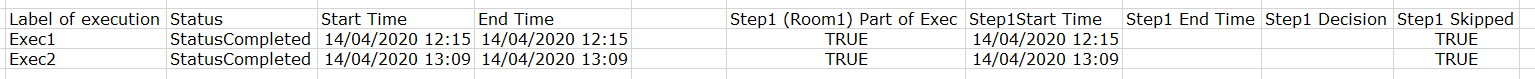
\includegraphics[width=\textwidth]{images/export_template.png}
	\centering
	\caption{Template-Sheet eines Excel-Exports}
	\label{fig:export-template}
\end{figure}

Für die Übersicht der Revisionen wird zusätzlich ein separates Sheet erstellt.
In dieses werden nach dem aufbereiten der Daten, in einer Tabelle die verschiedenen ursprünglichen Revisionen
mit ihren folgenden Revisionen gelistet.
Hier werden auch die erfassten Metriken dargestellt.
Dies resultiert in dem in \autoref{fig:export-orig-revisions} dargestellten Sheet.

\begin{figure}[htbp]
	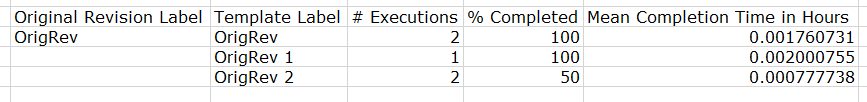
\includegraphics[width=\textwidth]{images/export_orig_revisions.png}
	\centering
	\caption{Ursprüngliche Revisionen-Sheet eines Excel-Exports}
	\label{fig:export-orig-revisions}
\end{figure}

Die daraus enstandene Excel-Datei ist immernoch nur im Hauptspeicher vorhanden
und muss auch nicht auf die Festplatte geschrieben werden.
Das Objekt der Datei kann auf ein \enquote{io.Writer}-Interface,
dass in der Standardbibliothek von Go enthalten ist, schreiben.
Dadurch kann das Objekt direkt in die Antwort der \gls{REST}-Schnittstelle die Datei schreiben.

\subsection{Tests}

Wie in allen Software-Projekten ist es wichtig, den Paper-Tracker zu testen.
Dabei spielt vor allem der Backend-Server ein große Rolle, da dieser die meiste Geschäftslogik implementiert.

Alle für den Server existierenden Tests sind automatisierte Tests, die einzelne Einheiten des Codes testen.
Vor allem werden die Manager getestet, da diese letzendlich die Geschäftslogik beinhalten.
Dafür werden verschiedene Bibliotheken verwendet.
Die \enquote{ginkgo}-Bibliothek stellt Funktionen zur Verfügung, um die Tests zu definieren
und Code vor/nach den Tests auszuführen.
Mit Hilfe von \enquote{gomega} können Ergebnisse der Tests mit zu erwartenden Ergebnissen verglichen werden.
Sie stellt neben den einfachen Vergleichen auch Vergleiche für Fehlertypen, komplexe verschachtelte Datenstrukturen,
Listen und mehr.

Damit die einzelnen Einheiten des Servers getrennt voneinander getestet werden können, wird zusätzlich die
\enquote{gomock} Bibliothek verwendet.
Diese ermöglicht es, Stellvertreterobjekte für in diesem Fall Manager und Repositories zu erstellen.
Die Stellvertreterobjekte können dann für jeden einzelnen Testfall mit zu erwarteten Parametern und einem Rückgabewert
konfiguriert werden.
Da \enquote{gomock} nur aus Interfaces Stellvertreterobjekte erstellen kann, müssen für alle Manager
und Repositories eigene Interfaces erstellt werden.
Deshalb gibt es, im Gegensatz zum Entwurf, für jeden Manager ein Interface und eine Implementierungsklasse.
Für die Tests wird dann die Instanz des Singletons auf ein Stellvertreterobjekt gesetzt.

Mit diesen Techniken wurden einige Tests für die Manager-, Modell- und Utilities-Klassen geschrieben.
Es sind somit ca. 20\% der Manager, ca. 27\% der Modelle und ca. 68\% der Utilities getestet. \TODO{MEHR!}

\section{Hardware und Firmware}

Im Folgenden wird erläutert, wie der Tracker hinsichtlich der verwendeten Hardware und der
entsprechenden Firmware implementiert wurde.

\subsection{Verwendete Technologien}

Als Mikrokontrollerplattform wurde die sogenannte \enquote{TinyPICO}-Plattform gewählt. Nach eigener
Aussage handelt es sich dabei um die kleinste vorgefertigte Entwicklungsplattform basierend auf
Mikrocontrollern vom Typ ESP32. Dieser Aspekt ist für die Erfüllung von \ref{nf:klein} wichtig.
Dieser Mikrocontroller wurde gewählt, da er alle benötigten Funktionen wie beispielsweise \gls{WLAN}
bereits über ein \gls{API} bereitstellt.

Die TinyPICO-Entwicklungsplattform stellt neben dem Mikrocontroller weitere Hardware bereit, so sind
unter anderem
die Stromversorgung über \gls{USB} sowie Lithium-Polymer-\gls{Akku}, ein Übersetzer von \gls{USB}
zu \gls{UART} zur Programmierung des Mikrocontroller und eine Vollspektrum-\gls{LED} verbaut.
Ein weiterer Vorteil ist das bereits integrierte Ladesystem, welches einen angeschlossen
Lithium-Polymer-\gls{Akku} automatisch auflädt, sobald der Tracker über \gls{USB} mit einer
Stromquelle verbunden wird. Außerdem können über das Ladesystem der aktuelle Ladezustand und die
Spannung des \gls{Akku} abgefragt werden, was für die Erfüllung von \ref{fa:benachrichtigung}
unabdingbar ist.

Die Firmware wurde in der Programmiersprache C++ auf Basis des Arduino-Frameworks erstellt. Dieses
Framework wurde gewählt, da es auf vielen Plattformen, wie auch dem ESP32 lauffähig ist, weit
verbreitet ist und somit viele Bibliotheken für das Framework existieren.

Das \enquote{Flasher}-Tool zum Programmieren und Konfigurieren der Firmware wurde in Python
entwickelt.
Der Grund dafür liegt in Möglichkeit sehr schnell und simpel ein Programm und auch ein \gls{GUI} zu
programmieren.
Dies wird durch die Bibliothek \enquote{PySimpleGUI} ermöglicht, die lediglich mit einer groben Layout-Beschreibung
ein Oberfläche zusammenstellt.
Alle weiteren benötigten Bibliotheken sind in der Python-Standardbibliothek enthalten.
Vor allem ist hierbei die \enquote{multiprocessing}-Bibliothek wichtig, mit welcher andere Programme aufgerufen werden können.
Um aus dem enstandenen Python-Skript eine ausführbare Datei für die verbreitesten Betriebssysteme zu erstellen, wird \enquote{PyInstaller} verwendet.
Die daraus enstehende Datei beinhaltet bis auf das PlatformIO-Tooling alle benötigten Ressourcen. \TODO{Kann man das mit bundeln?!}

\subsection{Flasher}
Aufgrund der angestrebten Einfachheit dieses Programmes, besteht es aus insgesamt nur drei Dateien.
Der Hauptbestandteil des Flashers ist das eigentliche Python-Skript.
Zusätzlich wird die Datei \enquote{requirements.txt} benötigt, welche alle Bibliotheken für den
Bibliotheksmanager \enquote{pip} auflistet.
In dieser Datei sind lediglich, wie oben erwähnt, \enquote{pysimplegui} und \enquote{pyinstaller} aufgeführt.
Die dritte und letzte Datei ist ein \enquote{Makefile}, welches einige Befehle zum Installieren der Bibliotheken,
Ausführen des Skripts oder Erstellen der ausführbaren Datei bereitstellt.

Das Skript selbst beginnt nach dem Importieren der benötigten Bibliotheken mit dem Parsen der
Kommandozeilenargumente.
Möglich ist nur das Argument \texttt{--keep-credentials}.
Das Skript erzeugt eine Datei, in welcher die Zugangsdaten für das vom Tracker zu verwendende
\gls{WLAN}-Netzwerk, sowie weitere potentiell sensitiven Informationen enthalten sind. Im
Standardfall wird diese Datei nach dem Erstelln der Firmware und der Programmierung des Trackers
gelöscht. Ist das Kommandozeilenargument \texttt{--keep-credentials} gegeben, wir die Datei nach
Erfolgreichem Abschluss des Programmiervorganges nicht gelöscht, was vor allem in der
Entwicklungsphase der Software vorteilhaft ist.

Weiter werden einige Konstanten definiert.
Diese sind zum einen der Titel des Programm-Fensters und einige sogenannte \enquote{Keys},
die eindeutig bestimmte Elemente der \gls{GUI} identifizieren.

Nach den Konstanten werden drei Funktionen definiert, die die eigentliche Logik des Flashers beinhalten.
Zuerst eine Funktion, die alle möglichen Ports, über die ein Tracker programmiert werden kann, auflistet.
Dies wird über ein Aufrufen von PlatformIO ermöglicht: \enquote{pio device list}.

Die nächste Funktion generiert die für die Firmware benötigte Datei mit der Konfiguration des Trackers.
Sie liest ein Template mit Platzhalter-Werten der Datei ein und ersetzt die Platzhalter mit den eingegebenen Werten, die als Parameter übergeben werden.
Nach dem Einsetzen der Werte, wird die Datei geschrieben.
Der Pfad, an dem sich die Firmware befindet, ist auch Teil der Werte, die als Parameter übergeben werden.
Zugriff auf einen einzelnen Wert wird über die oben erwähnten konstanten \enquote{Keys} ermöglicht.

In der letzten Funktion wird das Programmieren an sich ausgeführt.
Auch diese Funktion bekommt die eingebenene Werte als Parameter. Aus diesen wird der ausgewählte Port benötigt.
Mit diesem wird wieder PlatformIO aufgerufen: \enquote{pio run -e tinypico -t upload --upload-port port}.

Vor dem Hauptteil des Skripts werden noch die Layouts für die \gls{GUI} benötigt.
Es werden zwei verschiedene Layouts definiert: Ein Eingabe-Layout und ein Programmier-Layout.
Das Eingabe-Layout ist in \autoref{fig:flasher-input} dargestellt.
Es ist eine Tabelle aus Eingabe-Feldern mit Erklärungen, in denen alle benötigten Konfigurationen eingetragen werden können.
Die Eingabe-Felder selbst sind mit den Keys verknüpft.
Am unteren Teil des Layouts befindet sich ein Button, der das Programmieren startet.

\begin{figure}[htbp]
	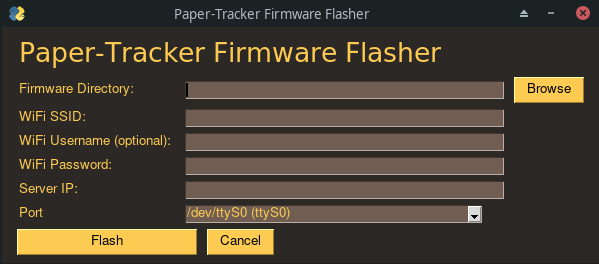
\includegraphics[width=\textwidth]{images/flasher/input.png}
	\centering
	\caption{Layout des Eingabe-Fenster}
	\label{fig:flasher-input}
\end{figure}

Das Programmier-Layout besteht lediglich aus einem Titel, einem Textfeld und einem Button.
Es ist in \autoref{fig:flasher-flash} dargestellt.
Im Textfeld soll der aktuelle Status angezeigt werden.
Der Button ist zum Schließen des Programms, sobald der Vorgang abgeschlossen ist.

\begin{figure}[htbp]
	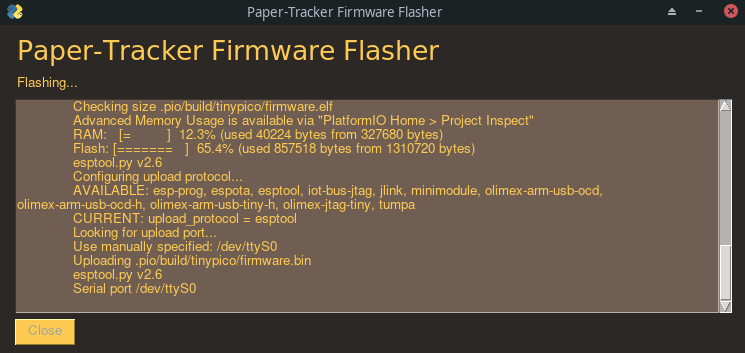
\includegraphics[width=\textwidth]{images/flasher/flash.png}
	\centering
	\caption{Layout des Programmier-Fenster}
	\label{fig:flasher-flash}
\end{figure}

Im Hauptteil des Skripts werden nun zuerst das Fenster mit dem Eingabe-Layout geöffnet.
Sobald der Button zum Start gedrückt wurde, werden die eingegebenen Werte ausgelesen.
Das Eingabe-Fenster wird geschlossen und das Programmier-Fenster mit den entsprechendem Layout geöffnet.
Ist dieses offen, wird die Funktion zum Generieren der Konfigurationsdatei und die Funktion zum Programmieren des Trackers aufgerufen.
Im Textfeld des Layouts werden diese Schritte entsprechend dokumentiert.
Auch die Ausgabe des Programmierens wird in das Textfeld ausgegeben.
Nach dem Programmieren wird, je nach Kommandozeilenargument, die generierte Datei gelöscht.
Nun kann das Fenster und damit das gesamte Programm über den Schließen-Button geschlossen werden.

Tritt während diesem gesamten Vorgang ein Fehler auf, wird dieser entsprechend aufgefangen und die Fehlermeldung im Textfeld angezeigt.
Das Löschen der generierten Datei wird auf im Fehlerfall ausgeführt.

\section{App}

Im diesem Kapitel wird die technische Umsetzung der App für Mobilgeräte beschrieben.

\subsection{Verwendete Technologien}

Zur Programmierung der App wurden die Programmiersprache Dart und das Framework Flutter verwendet.
Ein großer Vorteil dieser Kombination ist, dass Anwendungen sowohl für Android, als auch für iOS
kompiliert werden können, ohne den Quellcode anpassen zu müssen. Auch eine Laufzeitumgebung für
Desktopcomputer unter Windows, macOS und GNU/Linux befindet sich aktuell im Teststadium, sodass die
Paper-Tracker App gegebenenfalles auch auf Arbeitsplatzrechnern verwendet werden kann.

Auch für das Erstellen der App wurden einige Bibliotheken verwendet, die die Entwicklung vereinfachen.
Vor allem werden zum Beispiel Bibliotheken verwendet, um die Kommunikation mit dem Backend-Server zu ermöglichen.
Die verwendeten Bibliotheken sind im Folgenden aufgelistet:
\begin{description}
	\item[http (https://pub.dev/packages/http)] \hfill \\
		\enquote{http} ist eine Bilbiothek, die es ermöglicht asynchron \gls{HTTP}-Anfragen durchzuführen. Die Bibliothek wird dafür verwendet, um mit dem Backend-Server zu kommunizieren.
	\item[json\_annotation (https://pub.dev/packages/json\_annotation)] \hfill \\
		Mit \enquote{json\_annotation} kann über Annotationen im Programmcode eine Serialisierung zu JSON und Deserialisierung von JSON für Datenklassen generiert werden.
	\item[shared\_preferences (https://pub.dev/packages/shared\_preferences)] \hfill \\
		Durch die \enquote{shared\_preferences} Bibliothek können einfache Konfigurationen als Schlüssel-Wert-Paare abgespeichert werden. Dies wird für die \gls{URL} des Backend-Servers verwendet.
	\item[material\_design\_icons (https://pub.dev/packages/material\_design\_icons\_flutter)] \hfill \\
		\enquote{material\_design\_icons} stellt zusätzliche Material\footnote{Eine Designsprache von
			Google, die in fast allen Google-Produkten eingesetzt wird und auf Minimalismus setzt.
			\cite{Google2020}}-Icons zur Verfügung. Dies ist notwendig, da die standardmäßig verfügbaren Icons in Flutter nicht ausreichend sind.
	\item[fluttertoast (https://pub.dev/packages/fluttertoast)] \hfill \\
		Mit \enquote{fluttertoast} können kleine Pop-ups dargestellt werden, die dem Nutzer der App einfach und schnell Feedback zu einer Aktion geben können.
	\item[url\_launcher (https://pub.dev/packages/url\_launcher)] \hfill \\
		Mit Hilfe von \enquote{url\_launcher} können \gls{URL}s im Browser des Smartphones geöffnet werden. Für den Paper-Tracker wird dies zum Download des Daten-Export verwendet.
	\item[intl (https://pub.dev/packages/intl)] \hfill \\
		Die \enquote{intl}-Bibliothek wird für das Formatieren von Daten und Uhrzeiten verwendet. Zudem kann sie für die Übersetzung der App in andere Sprachen verwendet werden.
\end{description}

\section{Hardware-Gehäuse}

Neben der Hardware des spezifischen Trackers und der Software wurde auch ein Hardware-Gehäuse entwickelt.
Dieses Gehäuse soll den Tracker mit der Batterie beinhalten und eine Möglichkeit bieten, dieses an einem Stapel Papier zu befestigen.
Die Herstellung des Gehäuses soll in einem 3D-Drucker erfolgen.
Dazu muss das Gehäuse digital modelliert werden.

Bevor die Modelle selbst erstellt werden können, muss ein grobes Layout vorliegen.
Für den Paper-Tracker wurden zwei verschiedene Layouts in Betracht gezogen.
Diese werden in den folgenden Sektionen genauer erläutert und die aus den Layouts entstandenen Modelle gezeigt.

\subsection{Layout Controller auf der Batterie}
Das erste Layout ist in \autoref{fig:case-lay-on} abgebildet.
Bei diesem Layout befindet sich der Mikrocontroller auf der Batterie.

\begin{figure}[htbp]
	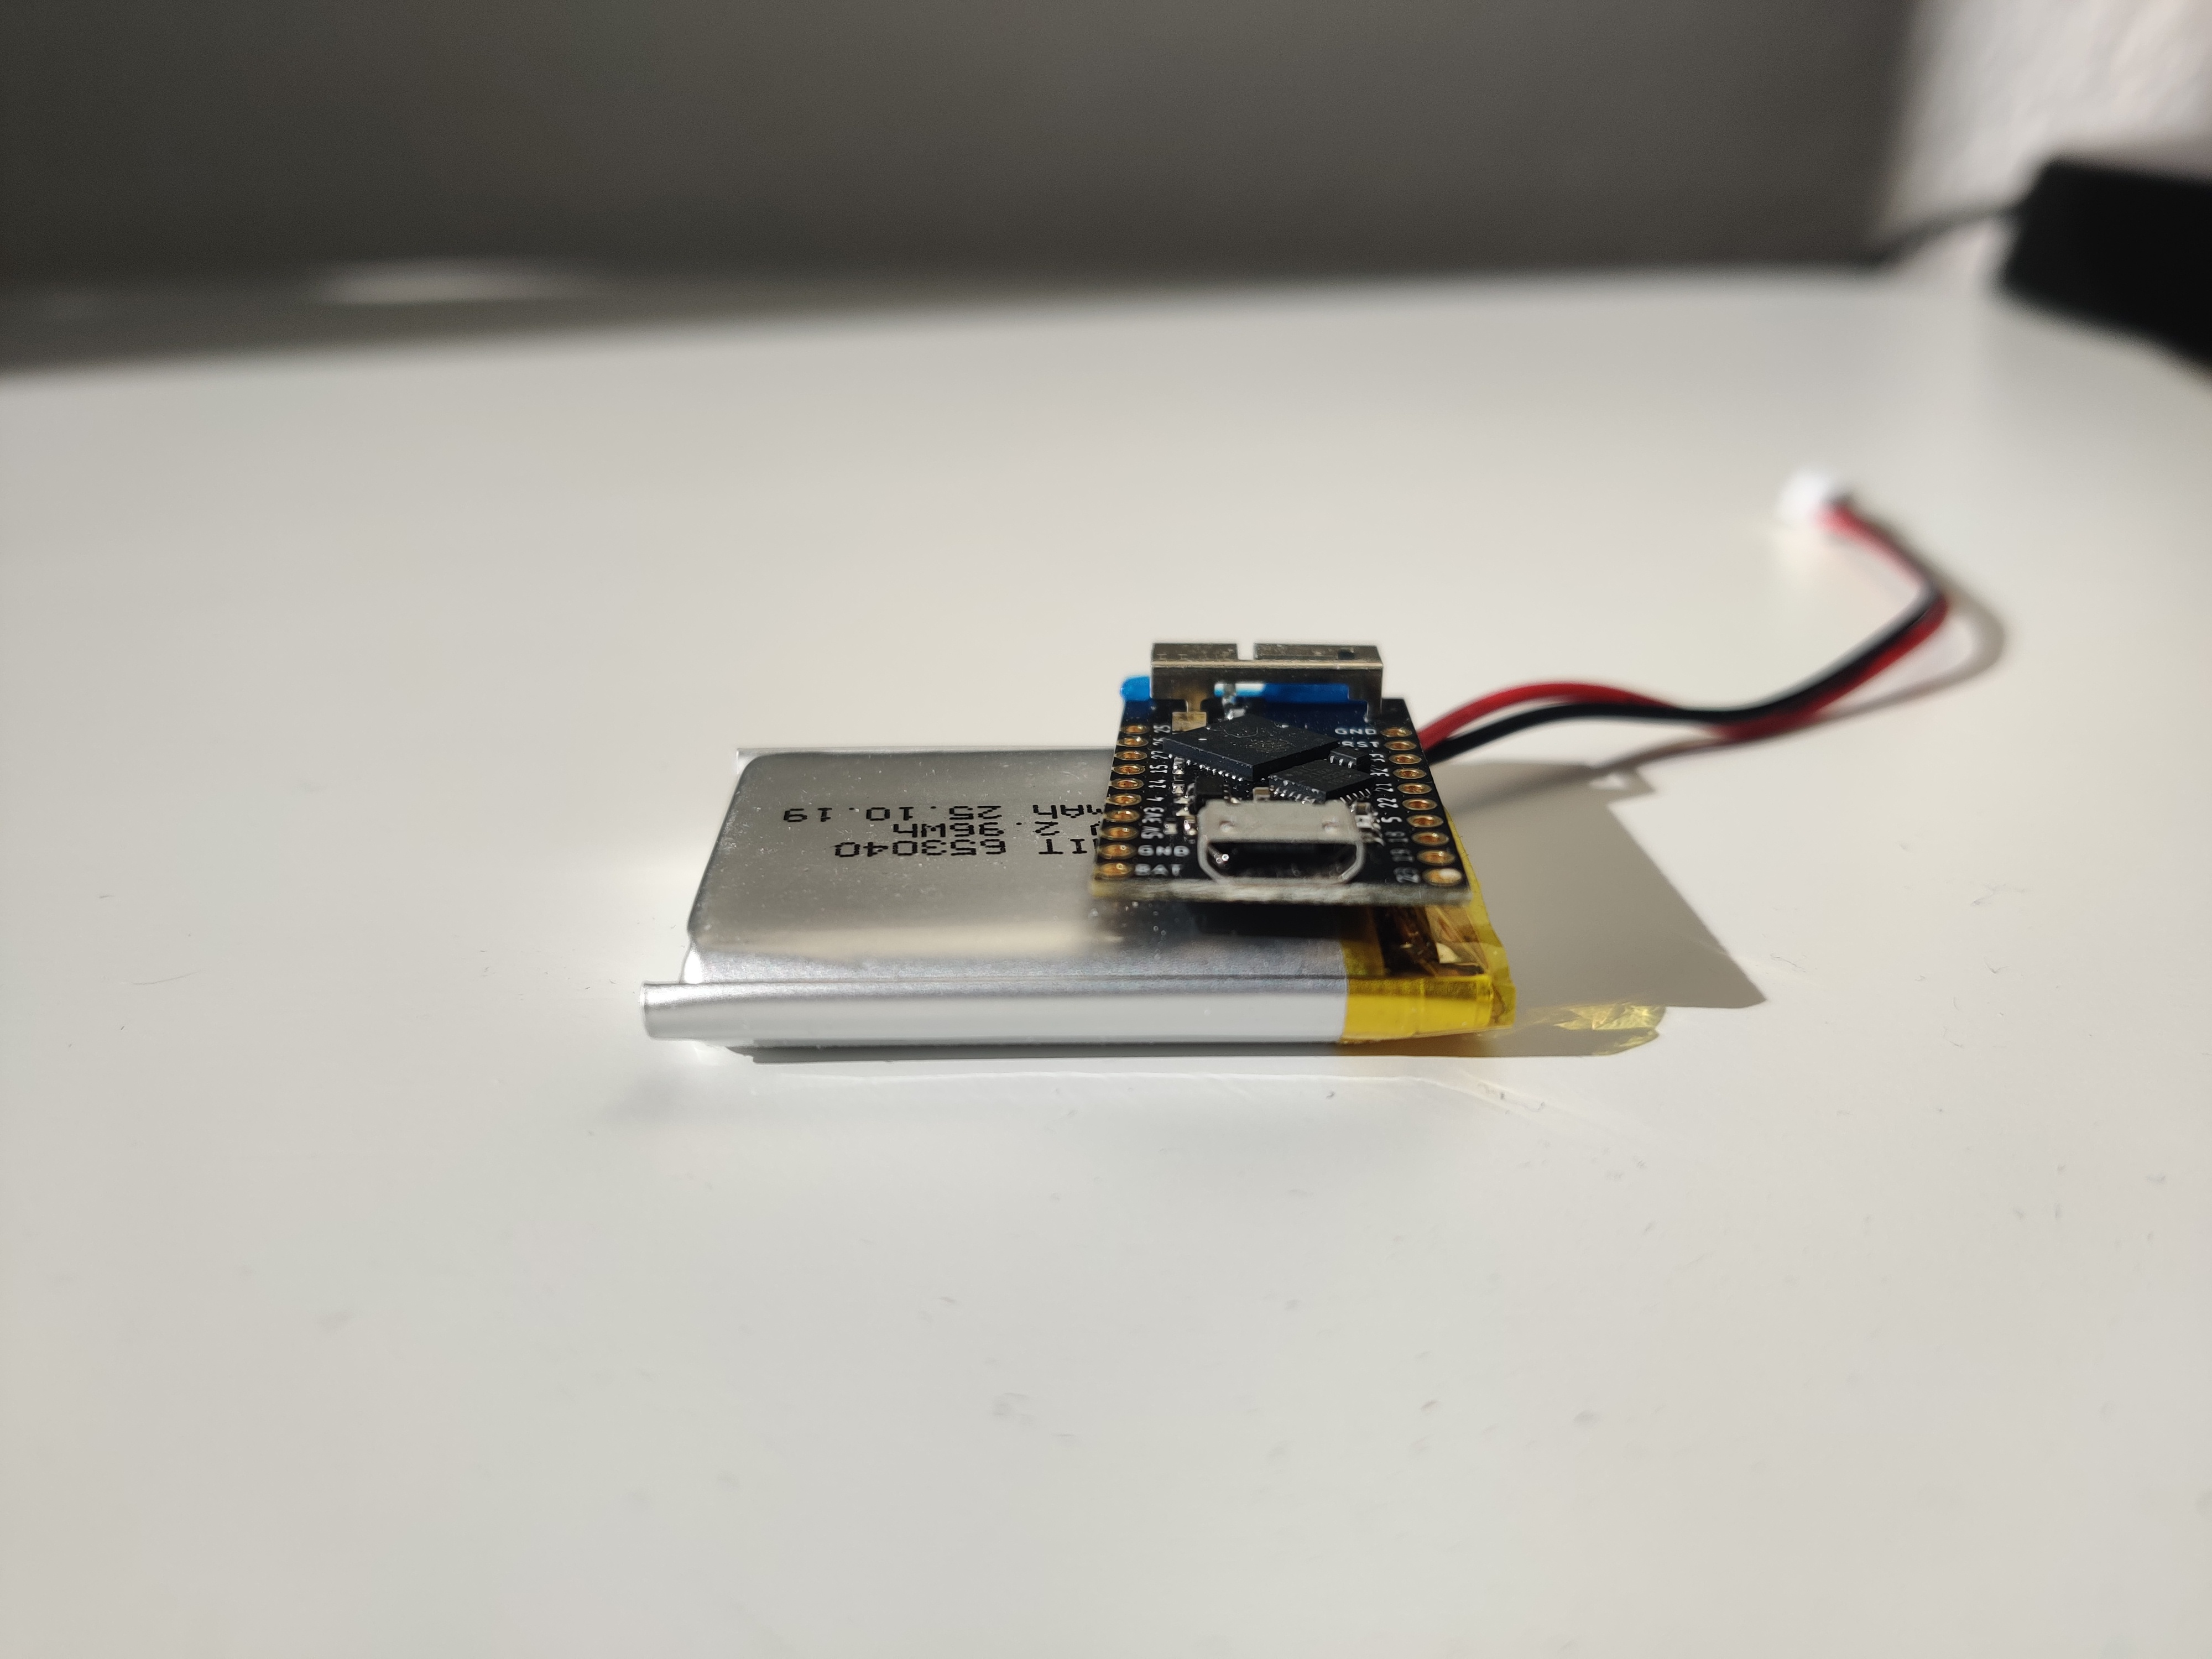
\includegraphics[width=300px]{images/case/pico_on_battery.jpg}
	\centering
	\caption{Gehäuse-Layout mit Mikrocontroller auf der Batterie}
	\label{fig:case-lay-on}
\end{figure}

Dies ergibt den Vorteil, dass die Grundfläche des Trackers mit ca. 45x35mm sehr gering gehalten wird.
Daraus ergibt sich dementsprechend der Nachteil, dass mit ca. 15mm die Konstruktion relativ hoch wird.

Das aus dem Layout enstandene Modell besteht aus zwei verschiedenen Teilen: Dem Körper des Gehäuse und dem Deckel.

Der Körper ist in \autoref{fig:case-high-body} dargestellt.
Er biete eine Art Schublade, in welche die Batterie hineinpasst.
Oberhalb der Schublade wird der Mikrocontroller durch Wände im Platz gehalten.
An der Seite gibt es eine Aussparung, um den \gls{USB}-Port zum Laden benutzen zu können.

Geschlossen wird der Körper mit dem Deckel.
Dies ist in \autoref{fig:case-high} dargestellt.
Die beiden Teile sollen nur über das Zusammenstecken miteinander verbunden werden.
Am Deckel ist auch der Mechanismus zum Anklemmen des Gehäuses an Papier angebracht.
Er besteht aus einem Steg, der schräg zum Gehäusekörper zeigt.
Zudem sind Noppen angebracht, die die Grifffestigkeit erhöhen sollen.

\begin{figure}[htbp]
	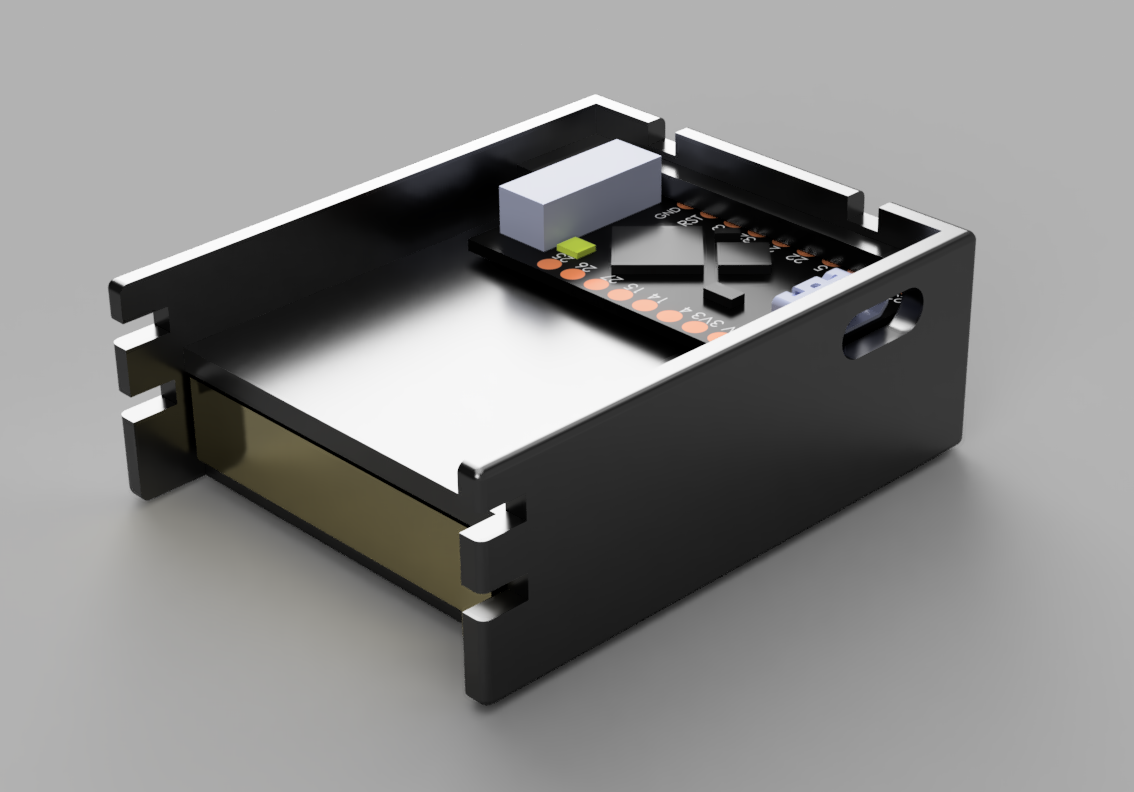
\includegraphics[width=300px]{images/case/high_body.png}
	\centering
	\caption{Körper des Gehäuse-Modell mit Controller auf der Batterie}
	\label{fig:case-high-body}
\end{figure}

\begin{figure}[htbp]
	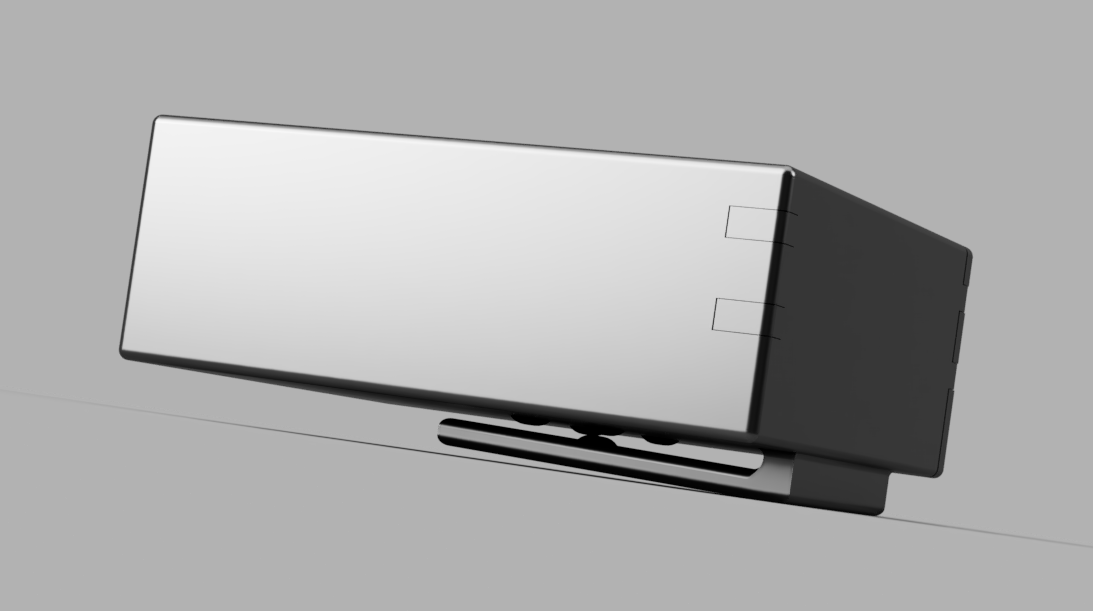
\includegraphics[width=300px]{images/case/high_complete.png}
	\centering
	\caption{Gehäuse-Modell mit Controller auf der Batterie}
	\label{fig:case-high}
\end{figure}

\FloatBarrier

\subsection{Layout Controller neben der Batterie}
Das zweite Layout ist in \autoref{fig:case-lay-beside} abgebildet.
Der Unterschied zum ersten Layout ist, dass der Mikrocontroller neben der Batterie platziert wird.

\begin{figure}[htbp]
	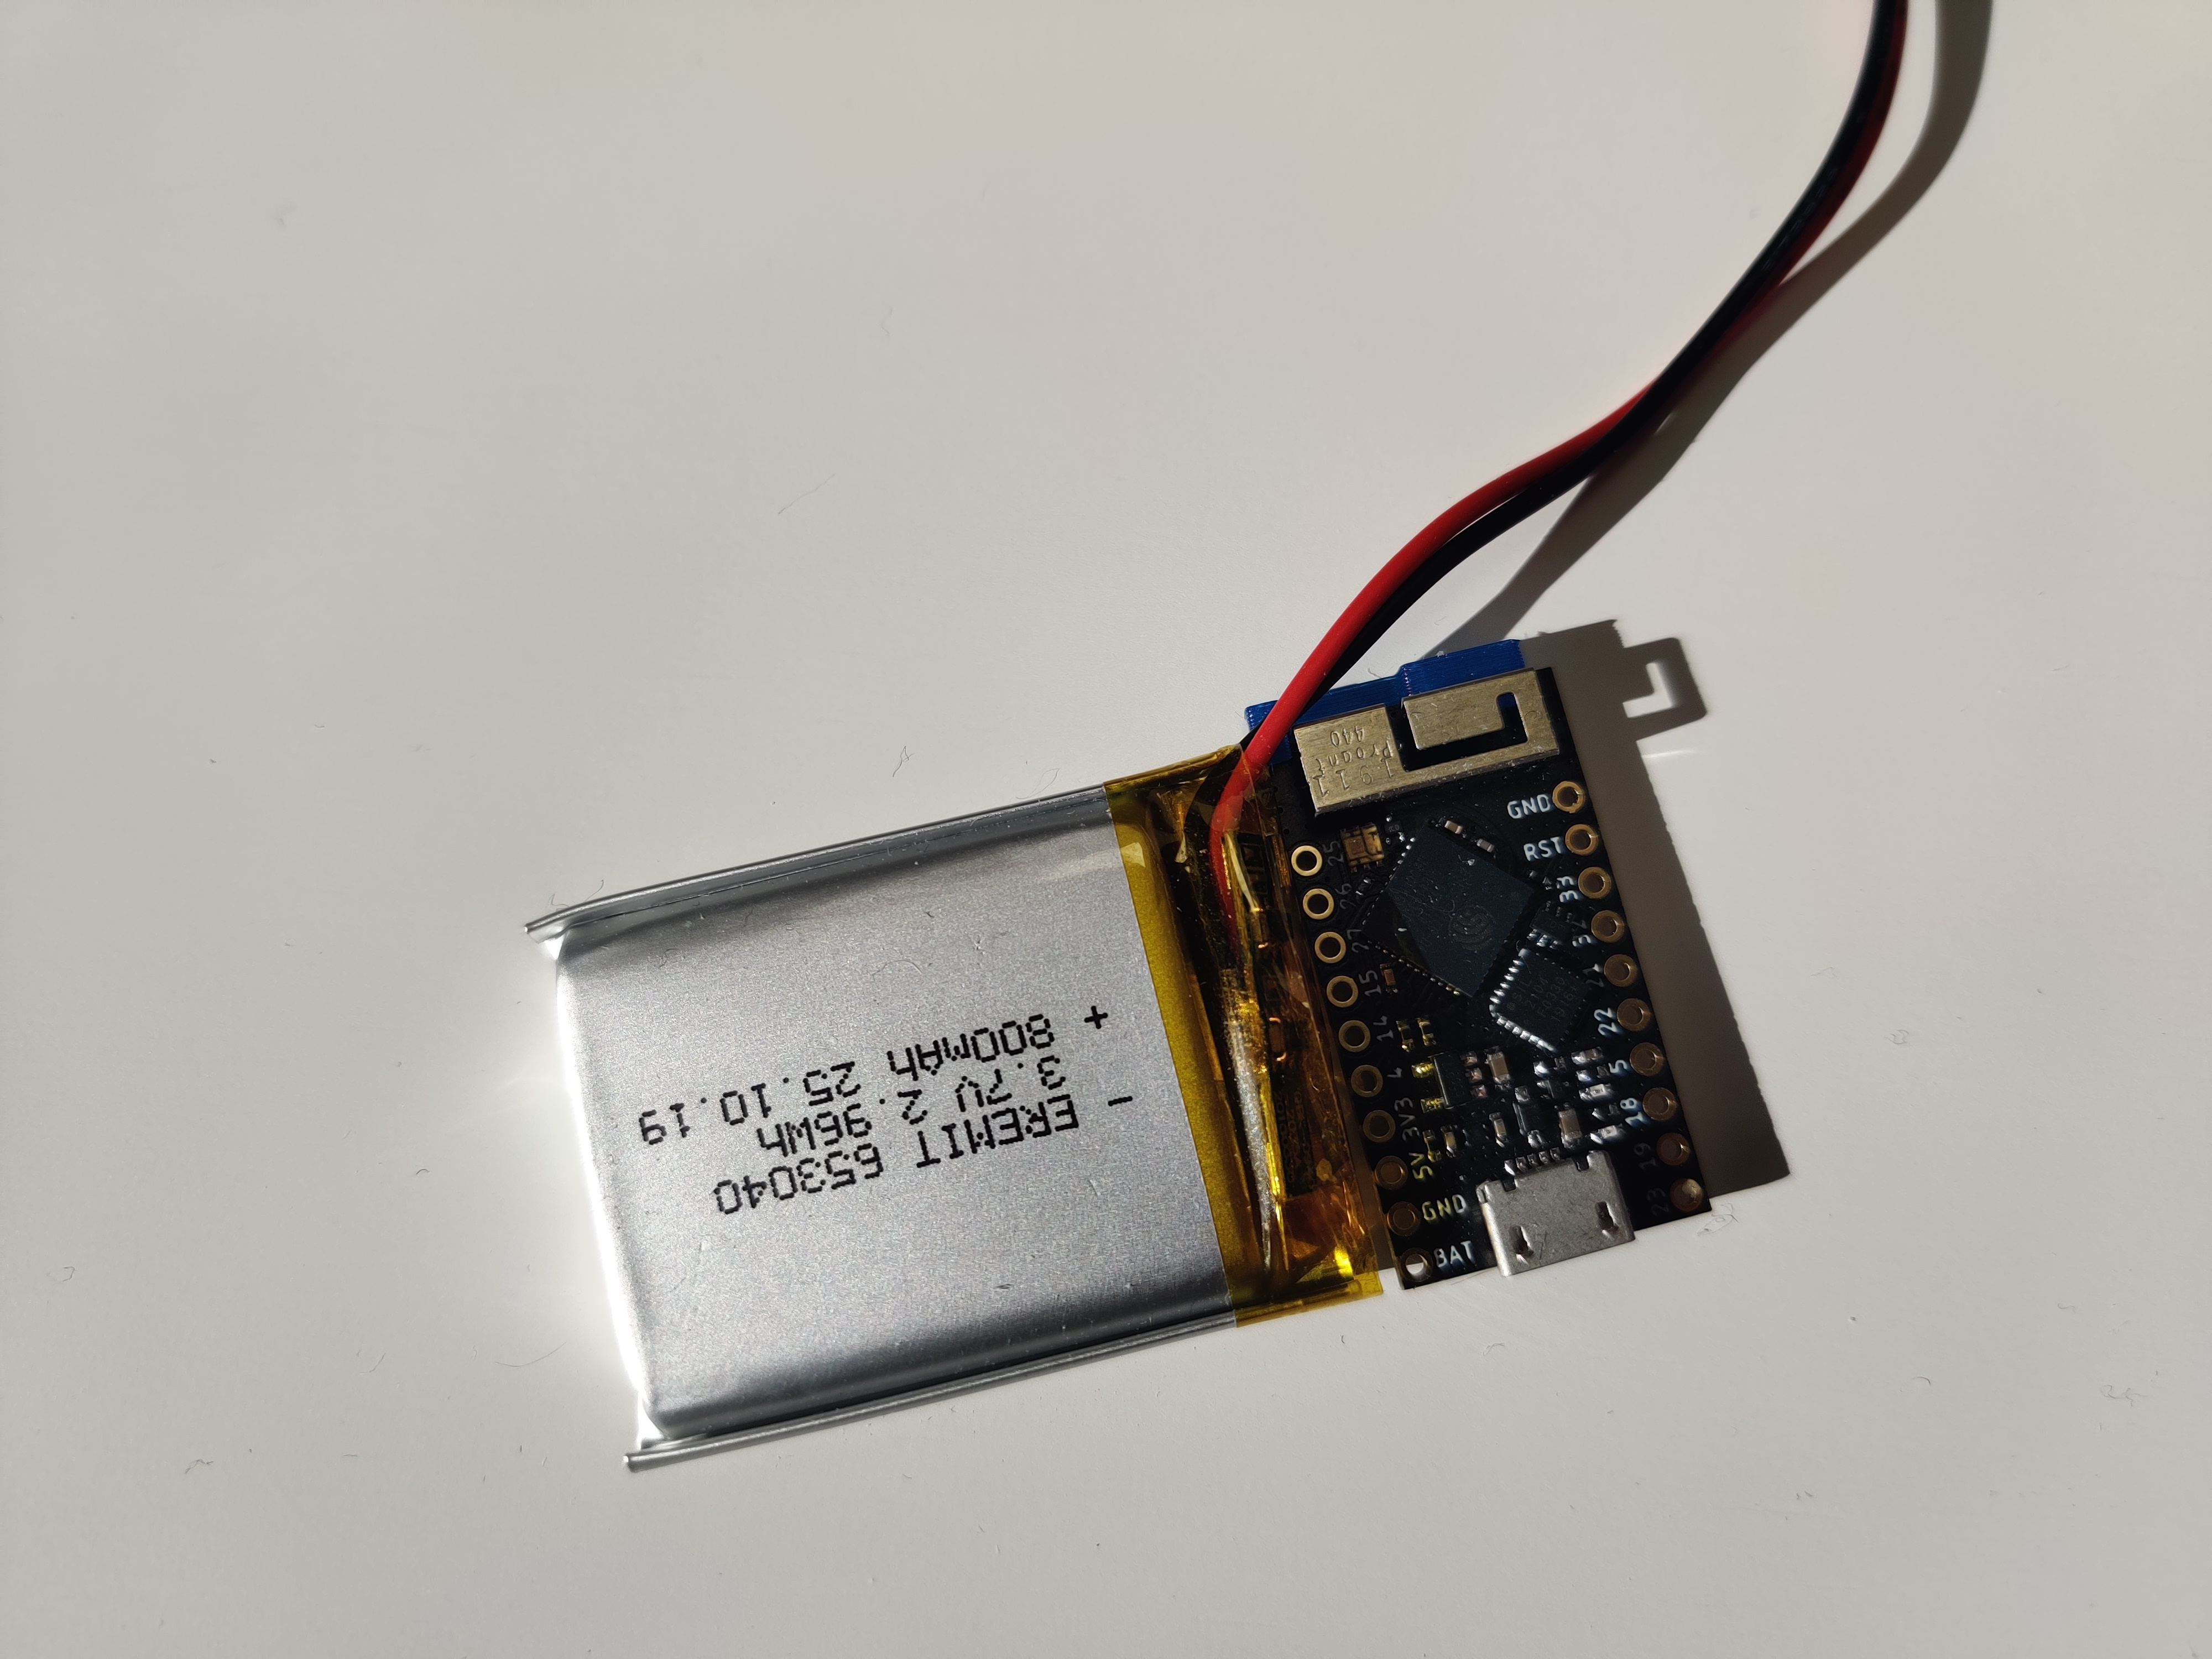
\includegraphics[width=300px]{images/case/pico_beside_battery.jpg}
	\centering
	\caption{Gehäuse-Layout mit Mikrocontroller neben der Batterie}
	\label{fig:case-lay-beside}
\end{figure}

Dies resultiert in einer erhöhten Grundfläche zum ersten Layout von 70x35mm aber in einer Reduktion der Höhe auf nur 12mm.

Das Modell nach diesem Layout ist in drei verschiedene Teile aufgeteilt.
Es gibt, wie zum ersten Layout, auch einen Körper und einen Deckel.
Zusätzlich gibt es jedoch noch den Clip zum Befestigen an Papier.
Dieser ist demnach nicht mehr im Deckel mit enthalten.

Der Körper ist in \autoref{fig:case-low-body} dargestellt.
Er bietet einen Platz für die Batterie und den Mikrocontroller nebeneinander.
Für den \gls{USB}-Port ist ebenfalls in der Außenwand eine Ausparung vorhanden.
Kleine Erhebungen halten die Teile am Platz und verhindern ein umherschieben.
In diesen Erhebungen sind auch Löcher für Schrauben inkludiert und auf der Unterseite Platz für eine Mutter.
Der größere Einschnitt in der Unterseite ist für den Clip bestimmt.

\begin{figure}[htbp]
	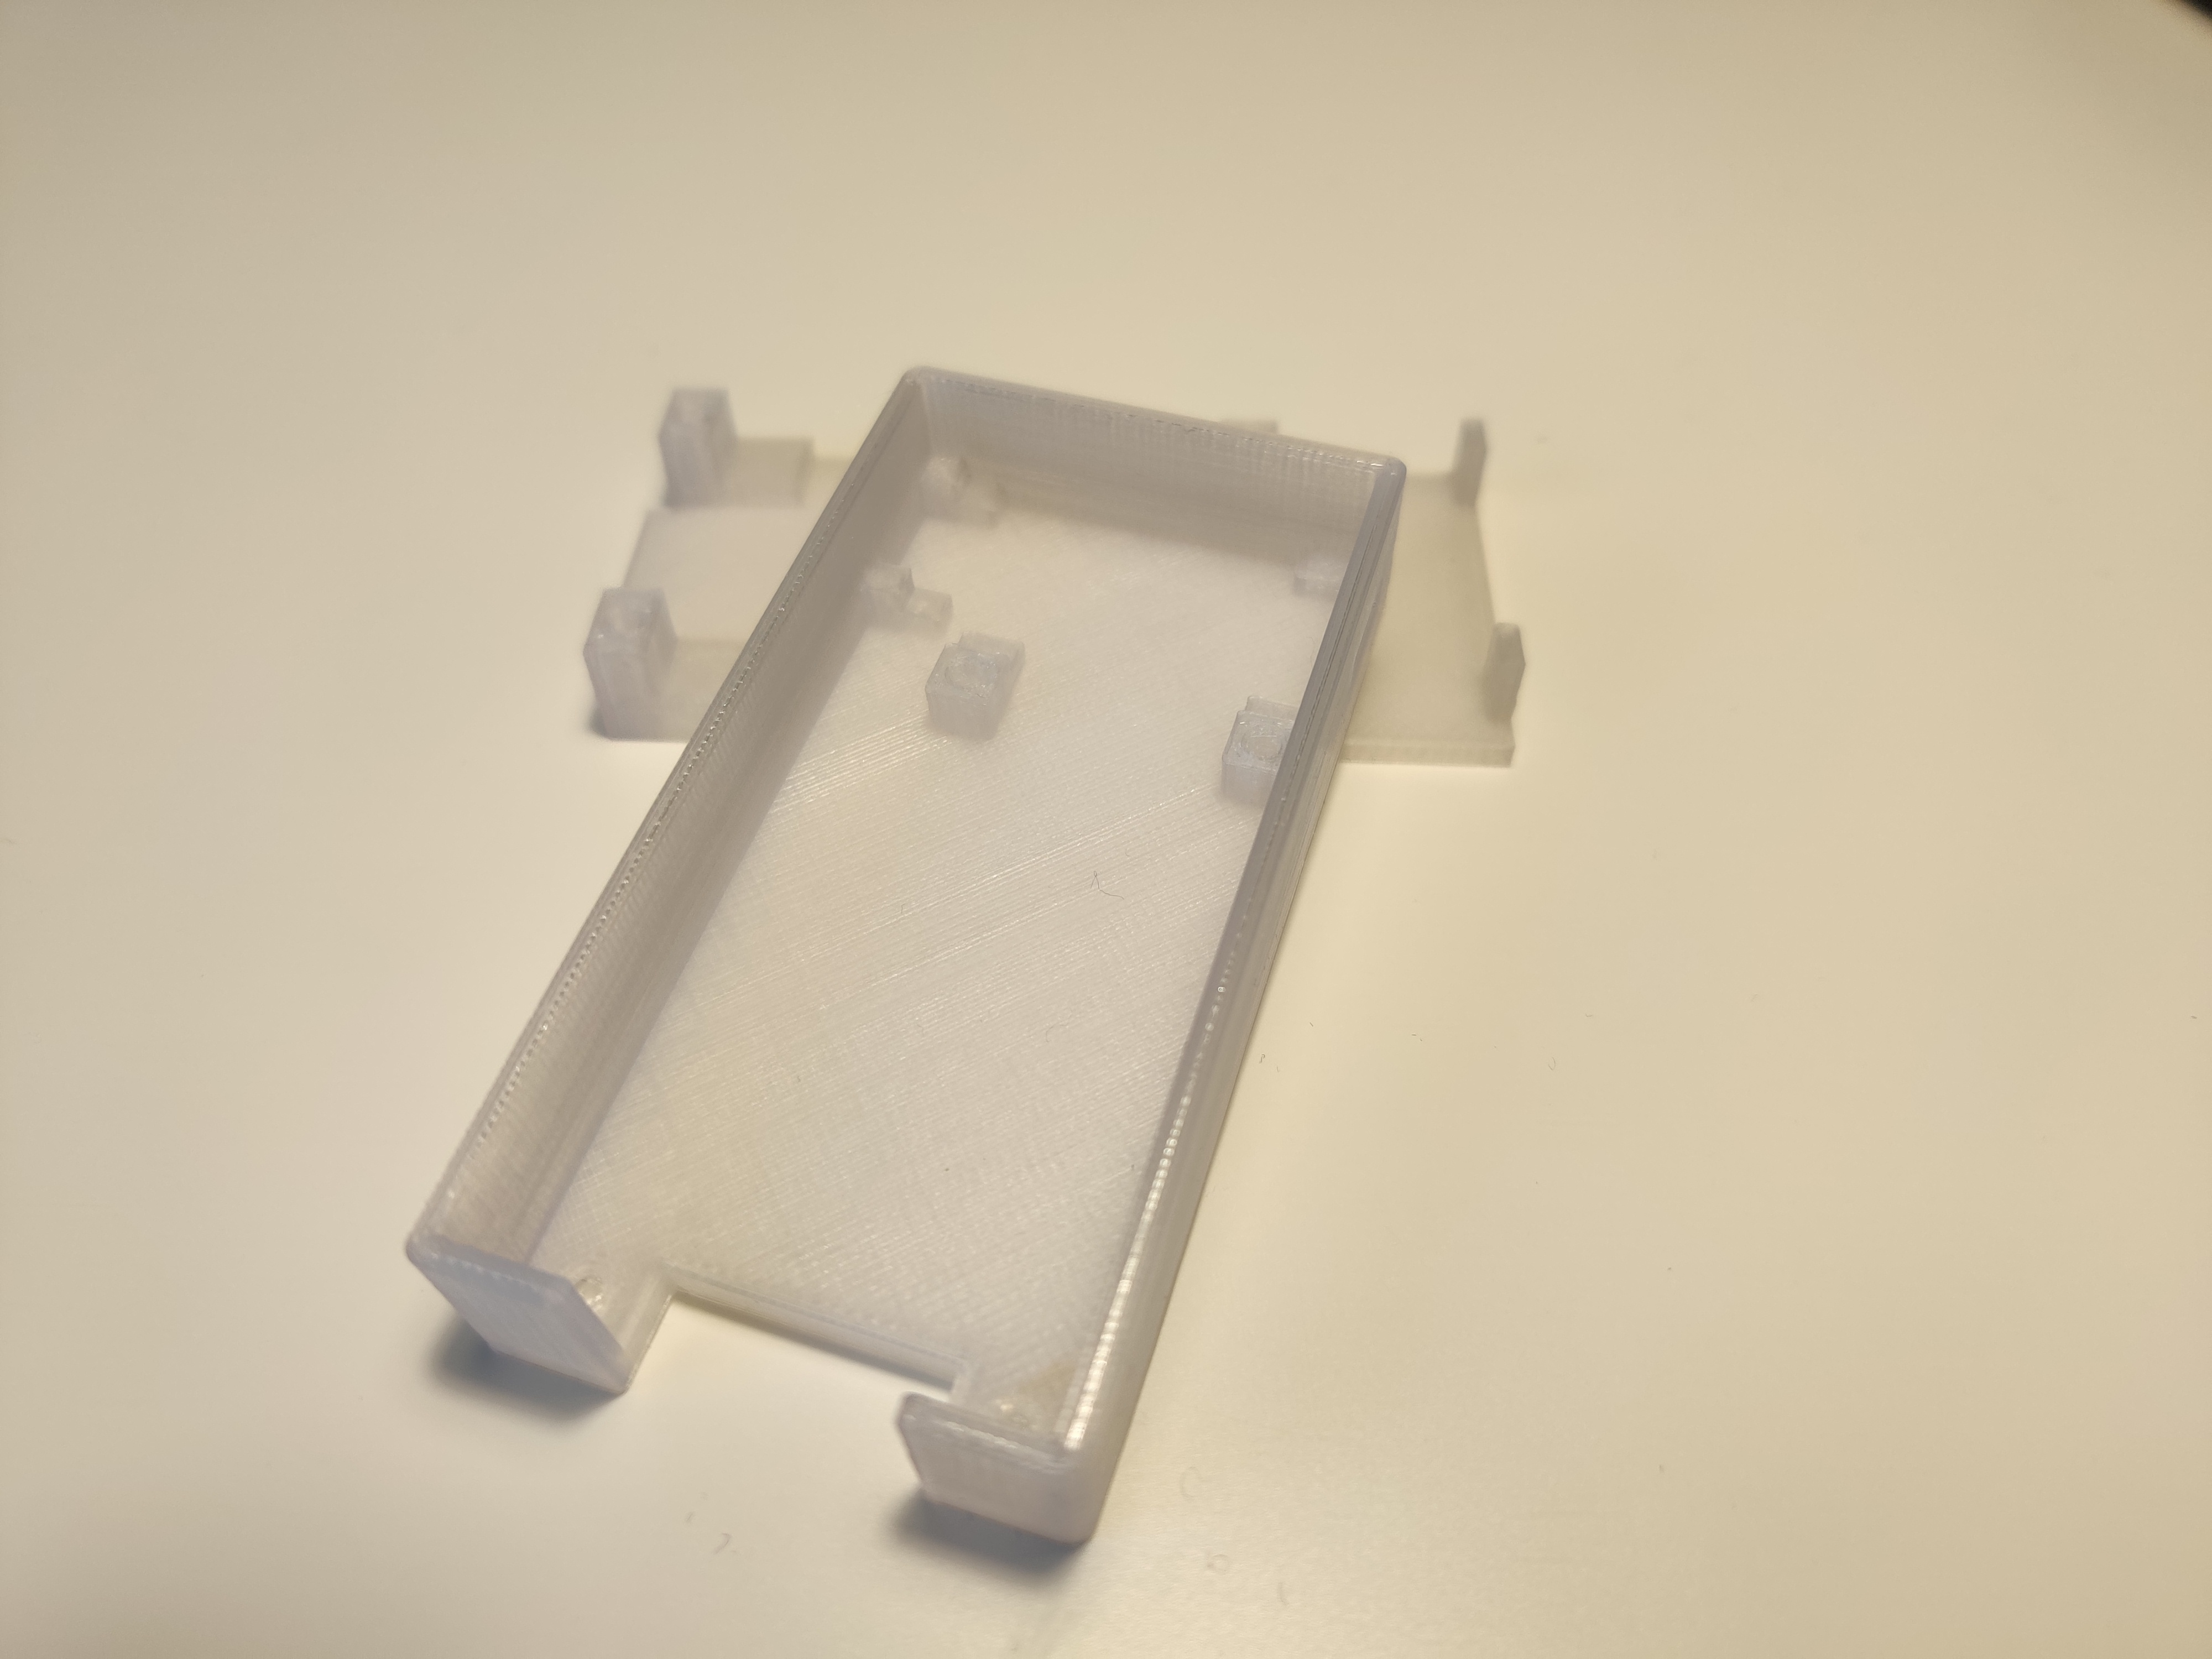
\includegraphics[width=300px]{images/case/low_body.jpg}
	\centering
	\caption{Körper des Gehäuse-Modell mit Controller neben der Batterie}
	\label{fig:case-low-body}
\end{figure}

Der Deckel des Modells ist ähnlich dem Körper, besizt aber keine Außenwände.
Er ist in \autoref{fig:case-low-lid} abgebildet.
Die kleinen Erhebungen des Deckels fixieren die Teile innerhalb des Gehäuses auf der vertikalen Achse.
Statt Platz für eine Mutter auf der Aussenseite der Erhebungen mit Schraubenlöchern, ist eine Einsenkung für den Schraubkopf vorgesehen.

\begin{figure}[htbp]
	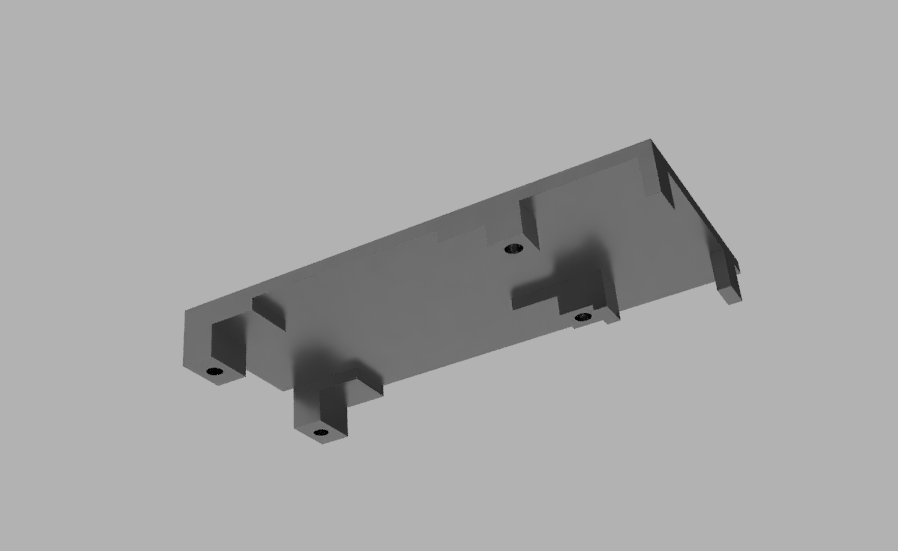
\includegraphics[width=300px]{images/case/low_lid.png}
	\centering
	\caption{Deckel des Gehäuse-Modell mit Controller neben der Batterie}
	\label{fig:case-low-lid}
\end{figure}

Angebracht ist der Clip an dem Einschnitt im Körper und fixiert durch die zwei danebenliegenden Schraubenlöcher.
Die Schraube wird dabei zwischen den Erhebungen des Körpers und des Deckels, sowie durch die in
\autoref{fig:case-low-clip} dargestellten Flügel des Clips geführt.
Für die Fixierung an einem Papierstapel wurde die gleiche Technik, wie für das erste Layout verwendet.
Um den 3D-Druck zu simplifizieren wurden bei diesem Entwurf jedoch keine Noppen an den Clip und an
den Körper des Gehäuses angebracht. Diese werden nach dem Druck aufgeklebt.

\begin{figure}[htbp]
	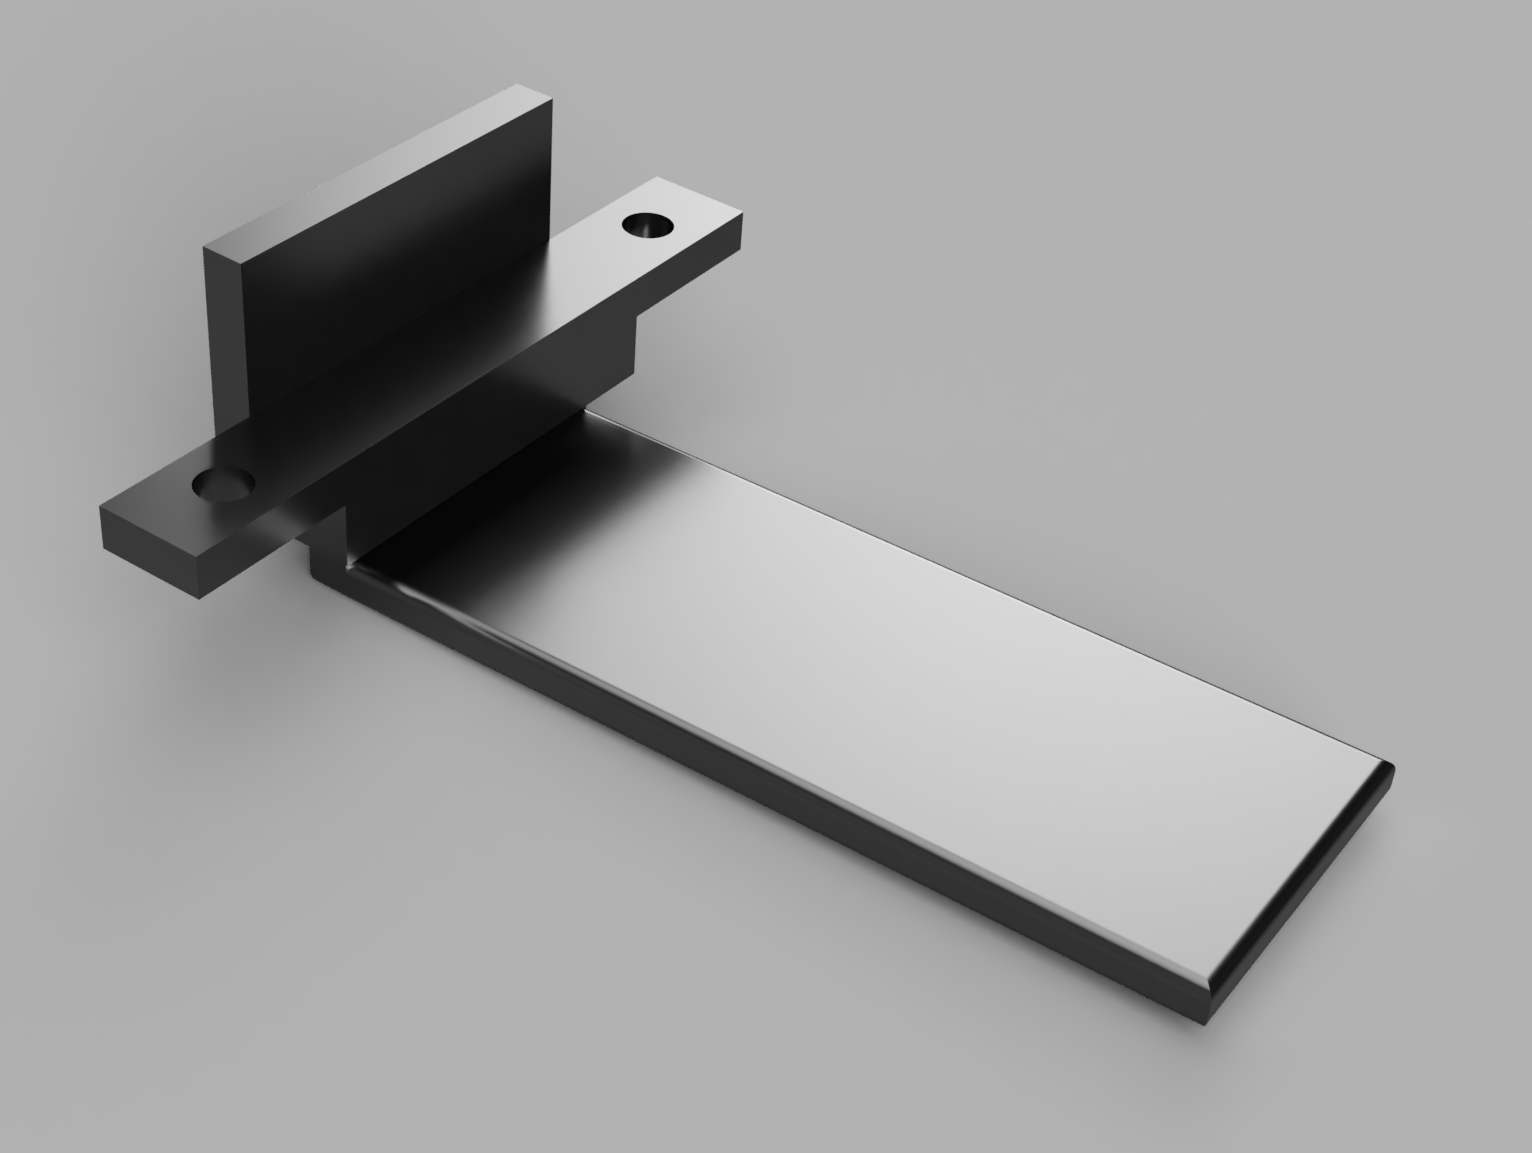
\includegraphics[width=300px]{images/case/low_clip.png}
	\centering
	\caption{Clip des Gehäuse-Modell mit Controller neben der Batterie}
	\label{fig:case-low-clip}
\end{figure}

\section{Bestehende Herausforderungen}
% Erstmal ein paar Beispiele
\subsection{Ungenauigkeit des Tracking}

\subsection{UI-Details in der App}
